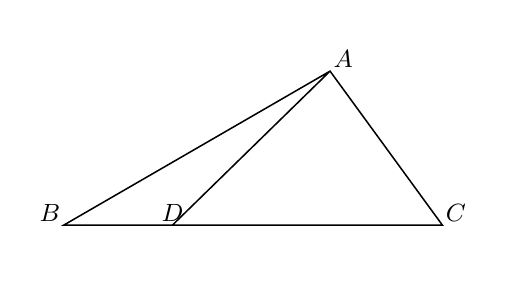
\begin{tikzpicture}[x=.023cm,y=-.023cm,baseline=(current bounding box.center),line width=.55pt,
  every node/.style={font=\small,inner sep=1pt}]
  \path[use as bounding box] (0,0) rectangle (250,136);
  \coordinate (B) at (20,109);
  \coordinate (C) at (229,109);
  \coordinate (A) at (167,24);
  \coordinate (D) at (80,109);
  \draw (B)--(A)--(C)--cycle (A)--(D);
  \node[above right] at (A) {$A$};
  \node[above left] at (B) {$B$};
  \node[above] at (D) {$D$};
  \node[above right] at (C) {$C$};
\end{tikzpicture}
